\documentclass[twocolumn]{article}

\usepackage{graphicx}
\usepackage{amsmath}
\usepackage{natbib}
\usepackage{geometry}
\usepackage{hyperref}
\usepackage{booktabs}

\geometry{margin=0.75in}

\title{LITTORAL: A Geometric Analysis of Global Relative Sea-Level Indicators Under Rotational Reorganization Hypotheses}
\author{Craig Stone}
\date{\today}

\begin{document}

\maketitle

\begin{abstract}
We present a global, geocoded compilation of relative sea-level (RSL) indicators---including submerged and raised beaches, reef terraces, sedimentary markers, and geomorphic shoreline features---assembled into the LITTORAL dataset. Spanning a vertical range of approximately $\pm 200$~m relative to present sea level, this dataset enables a geometry-first interrogation of global sea-level structure independent of conventional forward models. 

We compute the first-order spatial gradient of the LITTORAL elevation field and compare its structure to a pre-existing anisotropy field (the Mach field) derived from digital elevation model (DEM) flow alignment. The comparison reveals a non-random correspondence: preferred gradient pathways align with low-penalty Mach corridors, while high-penalty regions are systematically avoided. 

Conditioned discrimination tests, comparing observed candidate axes to matched random ensembles, demonstrate statistically significant reductions in integrated path penalties. These results support the hypothesis that global RSL indicators encode a coherent geometric structure consistent with large-scale redistribution processes. 

We interpret this structure in the context of geodetic sea-level change as described by \citet{fairbridge1961}, and explore its implications for rotational reorganization frameworks.
\end{abstract}

\section{Plain Language Summary}

Sea level is often treated as a simple global rise or fall. But the geological record tells a more complex story. Around the world, we find beaches, reefs, and shoreline features at many different heights---some far above today's oceans, others deeply submerged. 

In this study, we bring together thousands of these observations into a single global dataset and ask a different question: \emph{what shape do these data form?} Instead of assuming a cause, we examine the geometry directly.

We find that these sea-level markers are not randomly distributed. Instead, they follow preferred pathways across the Earth’s surface, forming a pattern that aligns with an independently derived global anisotropy field. This suggests that past sea-level changes may have been influenced by large-scale redistributions of mass or rotation, rather than purely local or gradual processes.

\section{Introduction}

The interpretation of relative sea-level (RSL) indicators has traditionally proceeded through forward models of eustatic change, glacio-isostatic adjustment (GIA), and tectonic uplift or subsidence. While these frameworks have achieved considerable explanatory power, they inherently impose causal structure prior to analysis.

An alternative approach is to treat the global distribution of RSL indicators as a geometric field and to interrogate its structure directly. This perspective aligns with the classical observations of \citet{fairbridge1961}, who emphasized that geodetic sea-level change may arise from redistribution of the Earth's mass and rotational geometry, rather than purely volumetric ocean change.

Fairbridge noted that:
\begin{quote}
Sea-level change is not simply a matter of adding or subtracting water, but involves the deformation of the geoid and the redistribution of the oceanic bulge under changing rotational conditions.
\end{quote}

This study revisits that perspective using modern data and computational tools. We assemble a global dataset of RSL indicators (LITTORAL) and examine its spatial structure through gradient analysis and comparison with an independently derived anisotropy field (the Mach field).

\section{Data: The LITTORAL Dataset}

The LITTORAL dataset comprises 3176 geocoded observations of relative sea-level indicators, compiled from published literature and databases including WALIS. Each record includes:

\begin{itemize}
\item Geographic coordinates (latitude, longitude)
\item Elevation or depth relative to present sea level
\item Indicator type (e.g., beach, reef, sedimentary marker)
\item Source reference
\end{itemize}

The dataset spans a vertical range of approximately $-200$~m to $+200$~m and provides global coverage across continental margins and ocean basins.

\begin{figure}[ht]
\centering
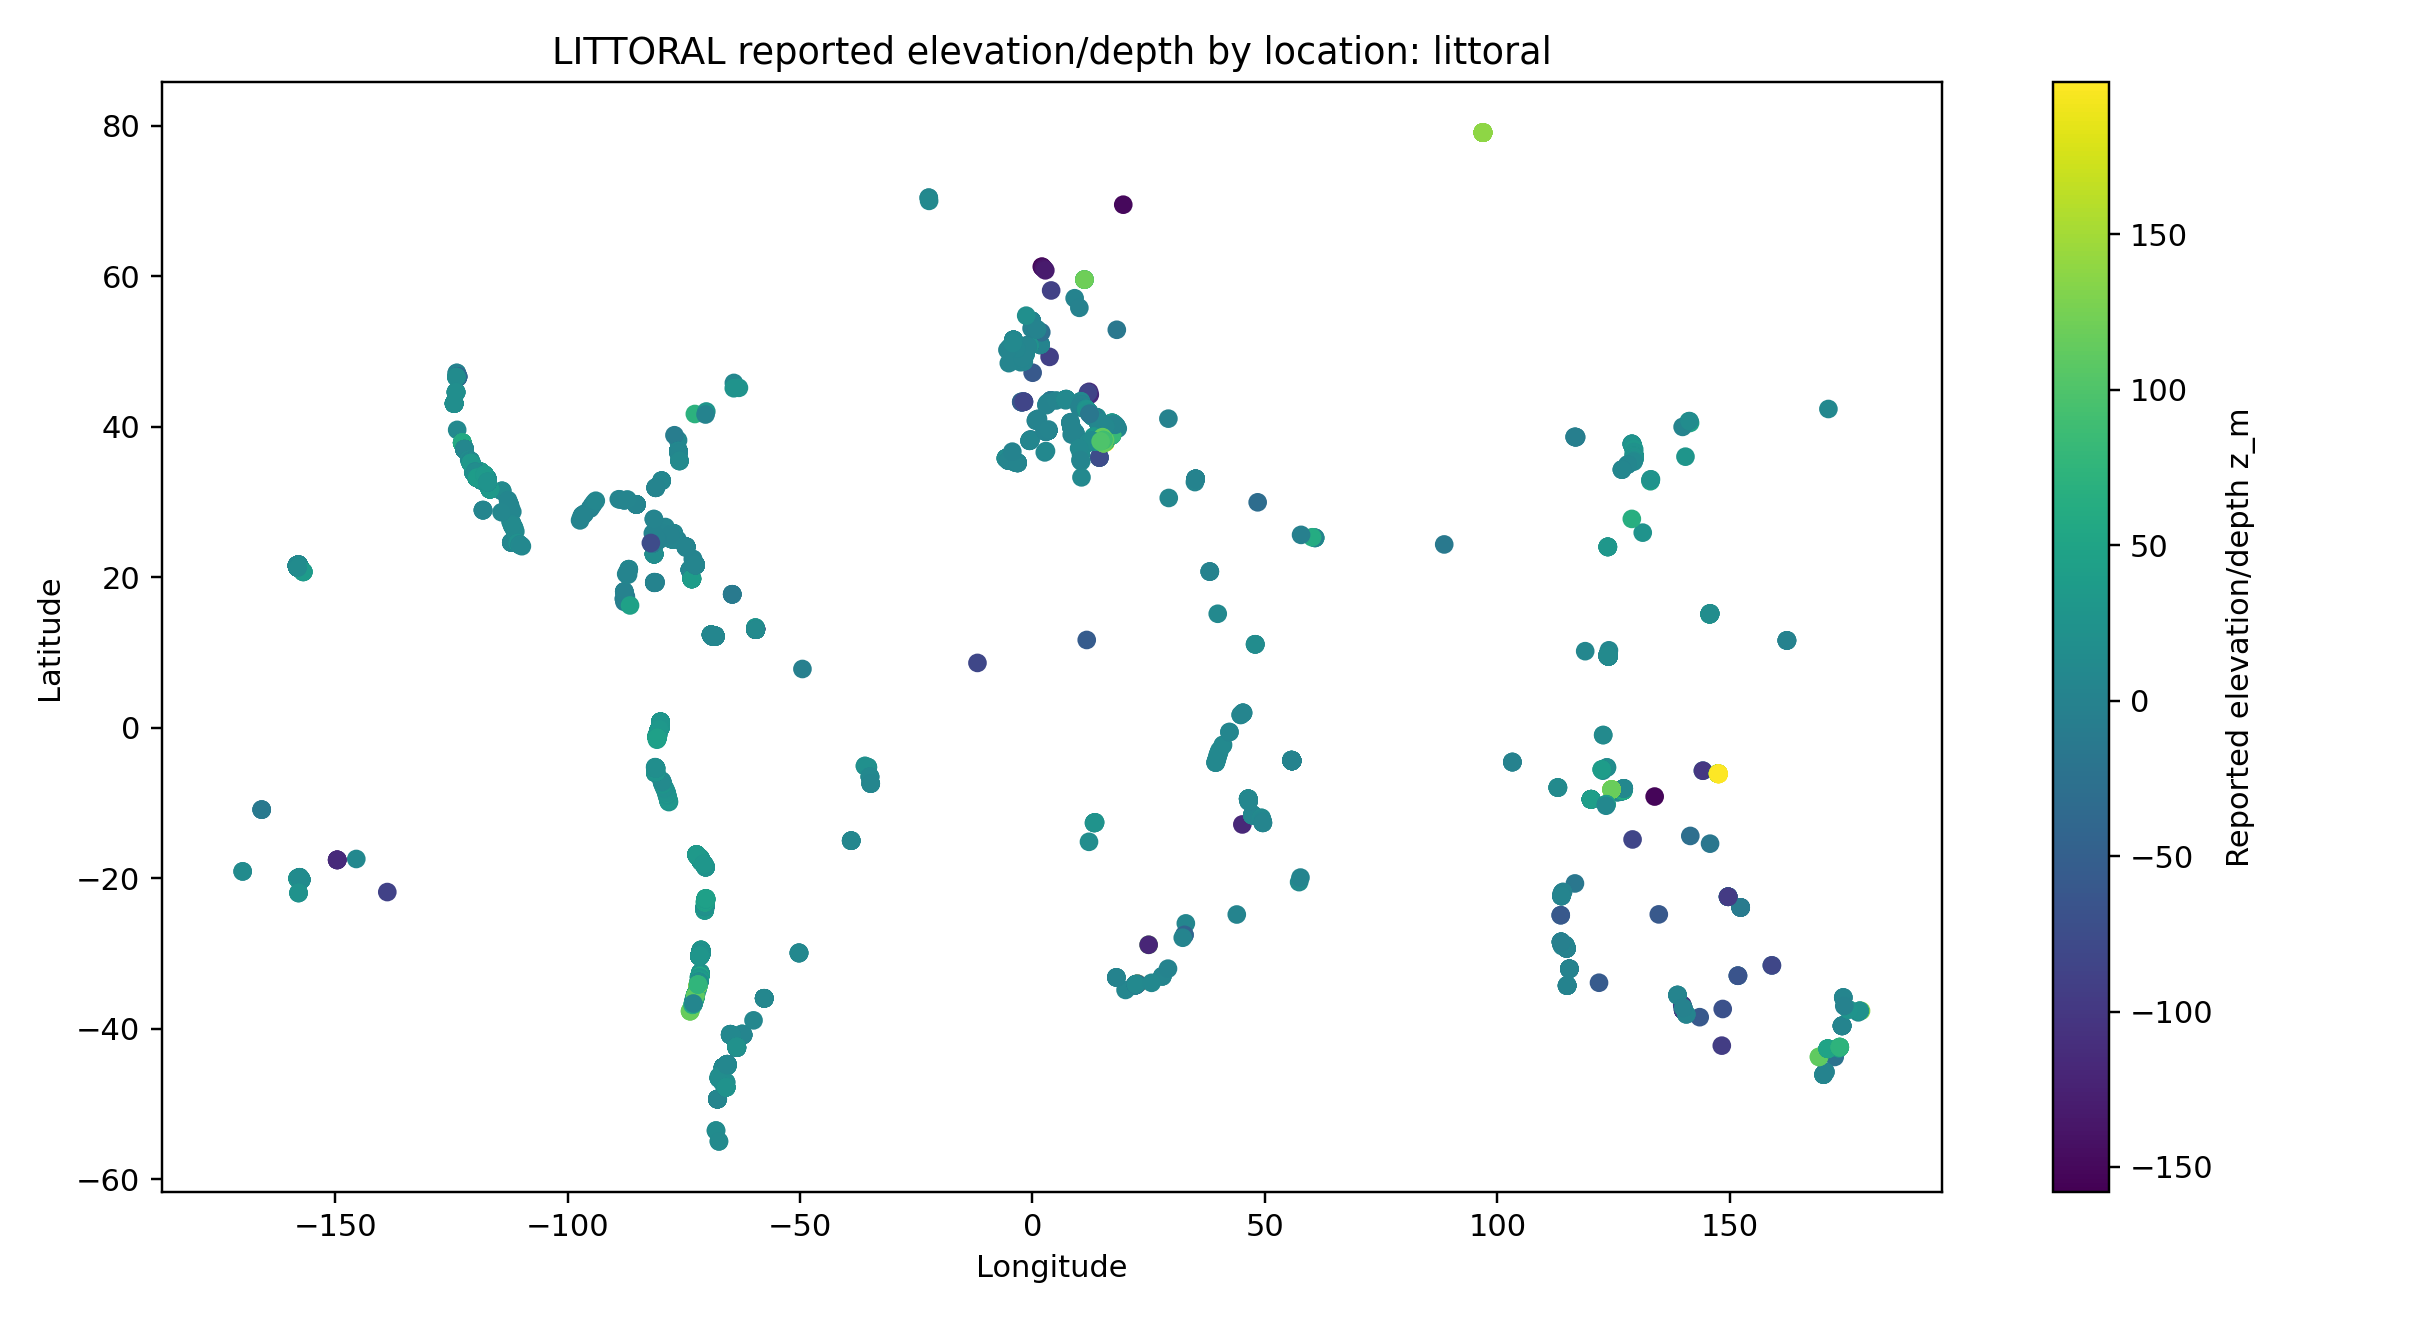
\includegraphics[width=\columnwidth]{outputs/geospatial_01/01_littoral_global_scatter_lon_lat_z.png}
\caption{Global distribution of LITTORAL dataset points, colored by elevation relative to present sea level. The dataset spans $\pm 200$~m and captures a wide range of coastal and marine indicators.}
\label{fig:dataset}
\end{figure}

\section{First-Order Gradient Structure}

To extract the large-scale spatial structure of the dataset, we compute the first-order gradient of the interpolated elevation field. This operation highlights directional trends and coherent pathways within the data.

\begin{figure}[ht]
\centering
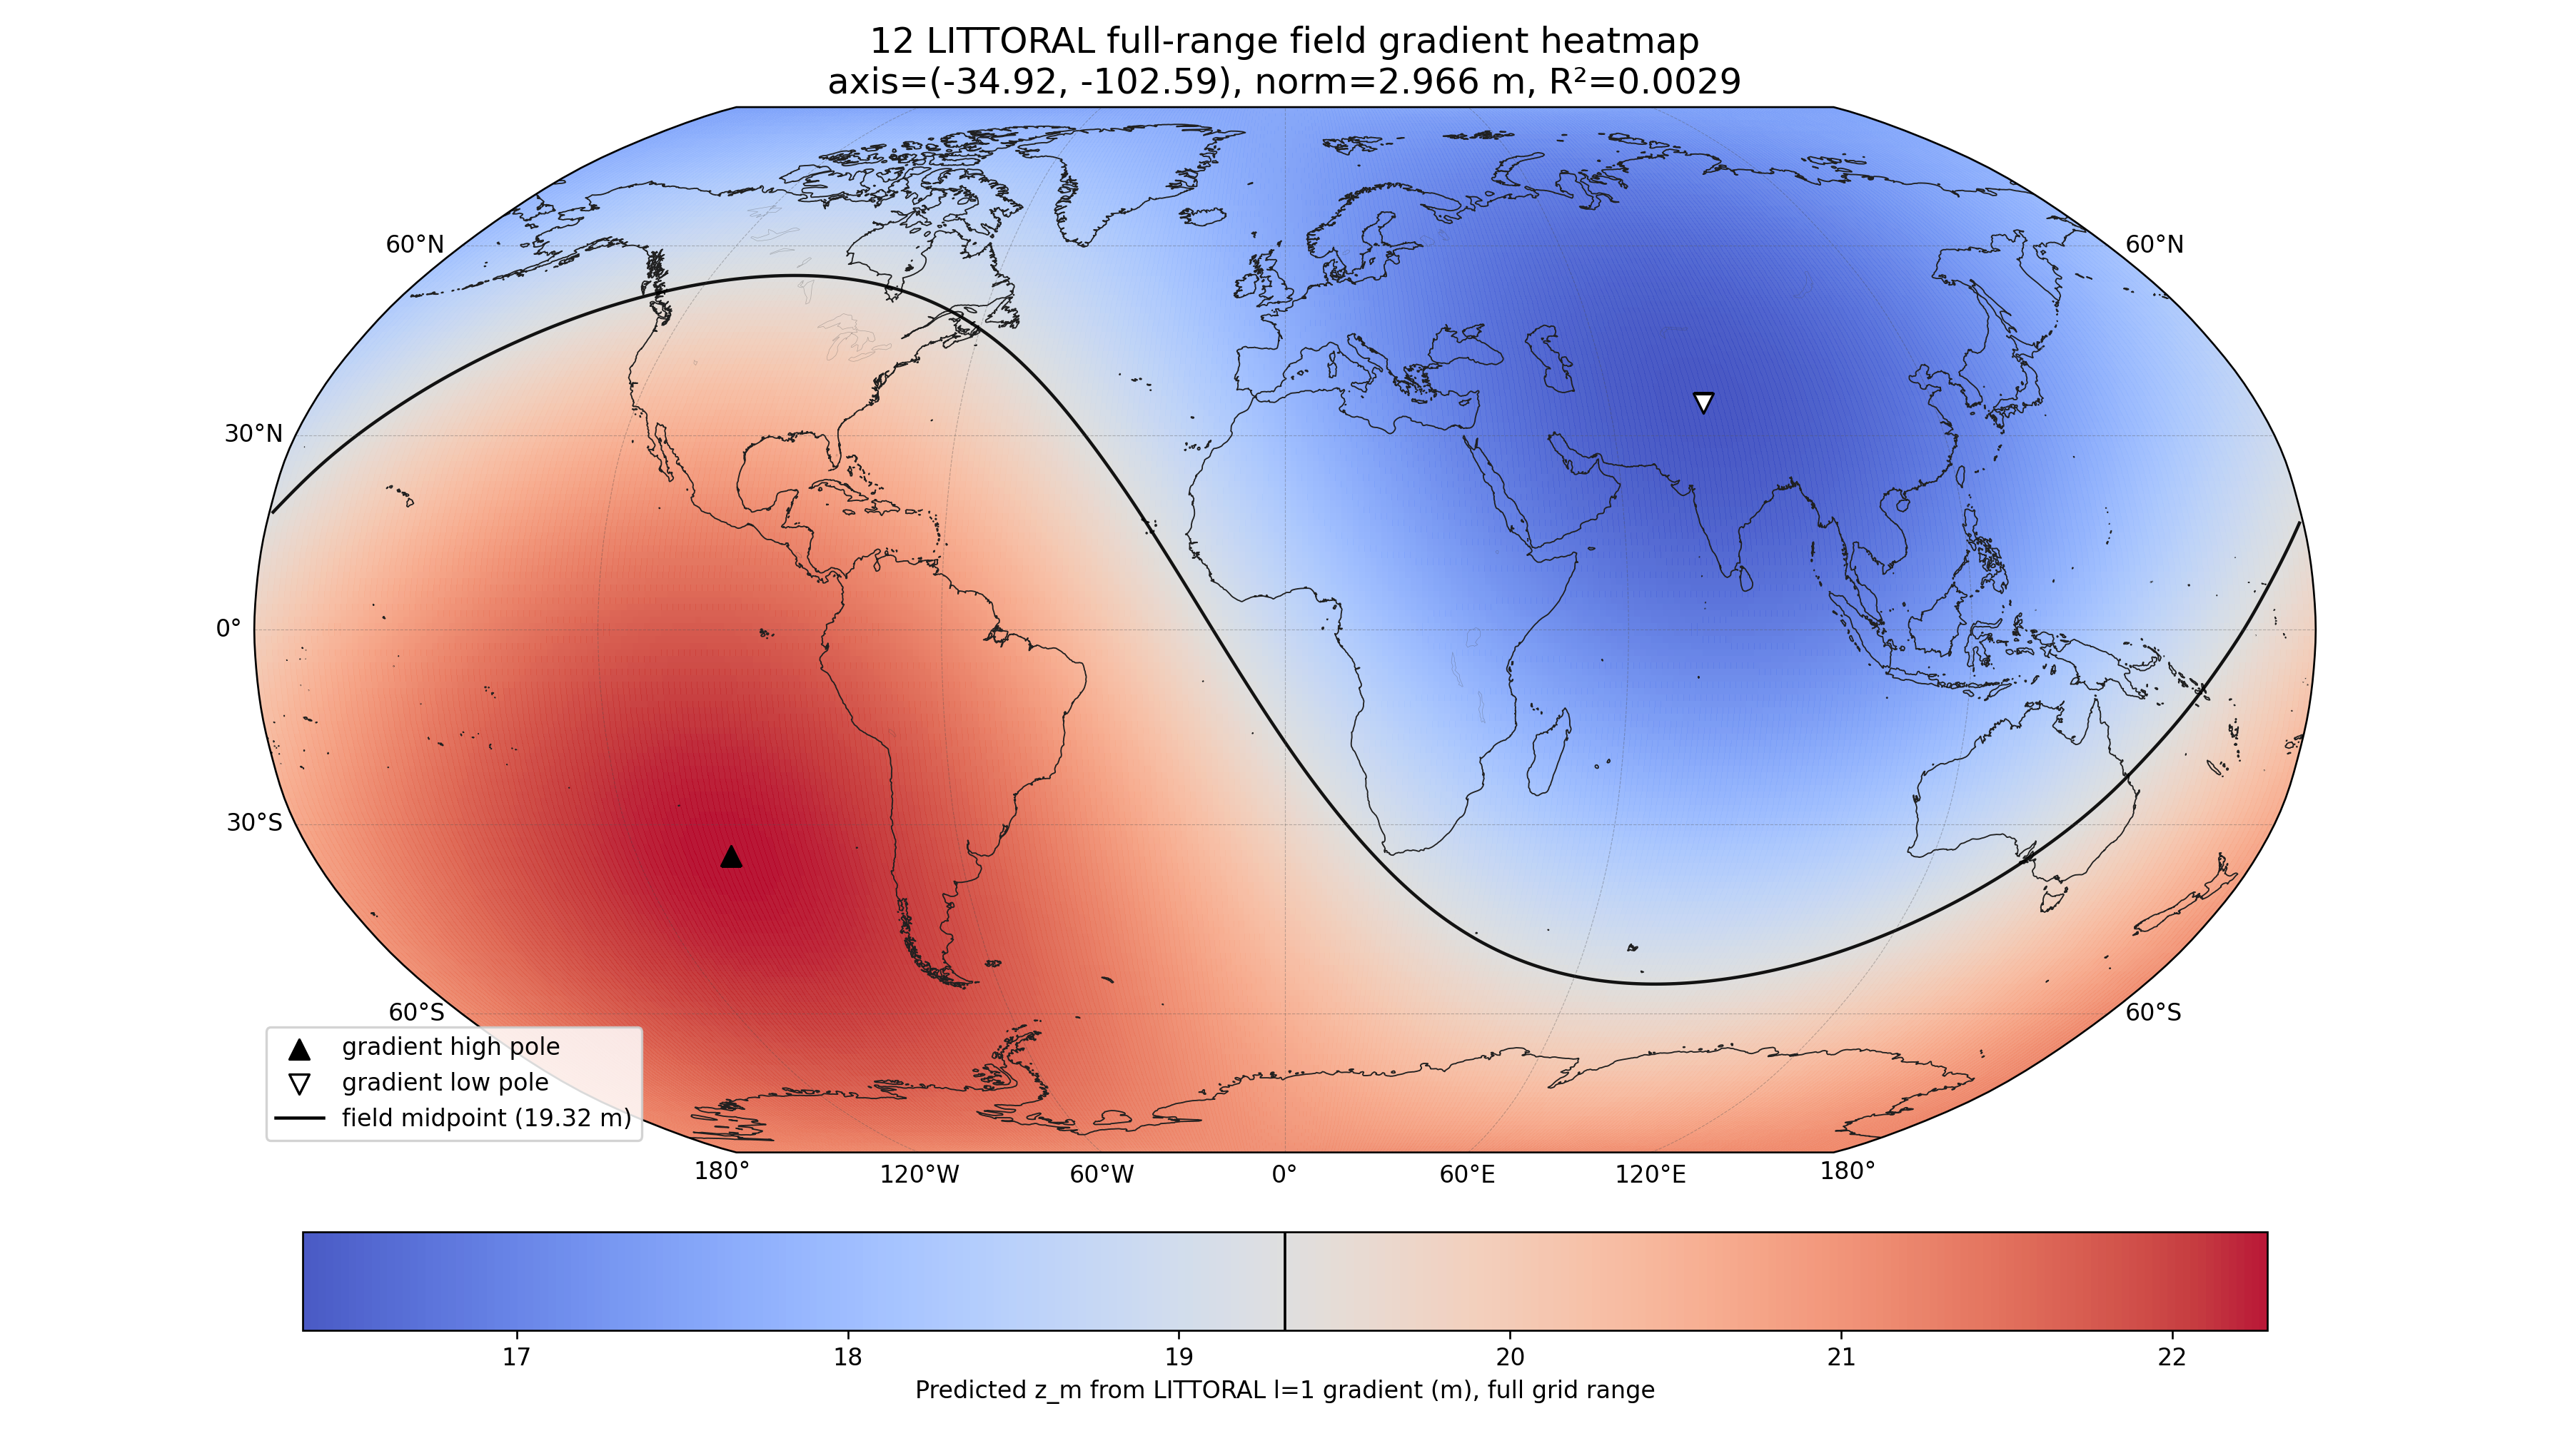
\includegraphics[width=\columnwidth]{outputs/geospatial_12/12_littoral_gradient_heatmap.png}
\caption{First-order spatial gradient of the LITTORAL elevation field. Coherent directional structures emerge, indicating preferred pathways in the global distribution of relative sea-level indicators.}
\label{fig:gradient}
\end{figure}

The resulting gradient field reveals pronounced anisotropy. Rather than exhibiting isotropic variation, the field organizes into bands and corridors, suggesting underlying geometric constraints.

\section{Conceptual Framework}

Following \citet{fairbridge1961}, we interpret these structures in terms of geodetic sea-level change. If the Earth's rotational configuration changes, the equilibrium shape of the ocean surface---the geoid---must adjust accordingly. This leads to redistribution of water masses and corresponding shifts in relative sea level.

In this framework, the observed elevation field is not simply a record of local uplift or subsidence, but a projection of a global geometric transformation.

The key question then becomes: \emph{does the observed structure align with an independently derived geometric field?}

\section{The Mach Field: A Reference Anisotropy}

To provide an independent geometric reference, we employ the Mach field---a global anisotropy metric derived from digital elevation model (DEM) analysis. The Mach field quantifies the compatibility between local topographic gradients and a prescribed global flow geometry, expressed in terms of an Euler rotation field.

Formally, the Mach metric $M$ evaluates the misalignment between the local surface gradient vector $\nabla h$ and the expected flow direction $\mathbf{v}_{\text{Euler}}$ at each point on the sphere:
\begin{equation}
M = 1 - \left| \hat{\nabla h} \cdot \hat{\mathbf{v}}_{\text{Euler}} \right|
\end{equation}
where hats denote unit vectors. Low values of $M$ indicate strong alignment (high compatibility), while high values indicate misalignment (low compatibility).

The resulting field partitions the Earth's surface into corridors of high and low geometric admissibility under the assumed rotational flow.

\begin{figure}[ht]
\centering
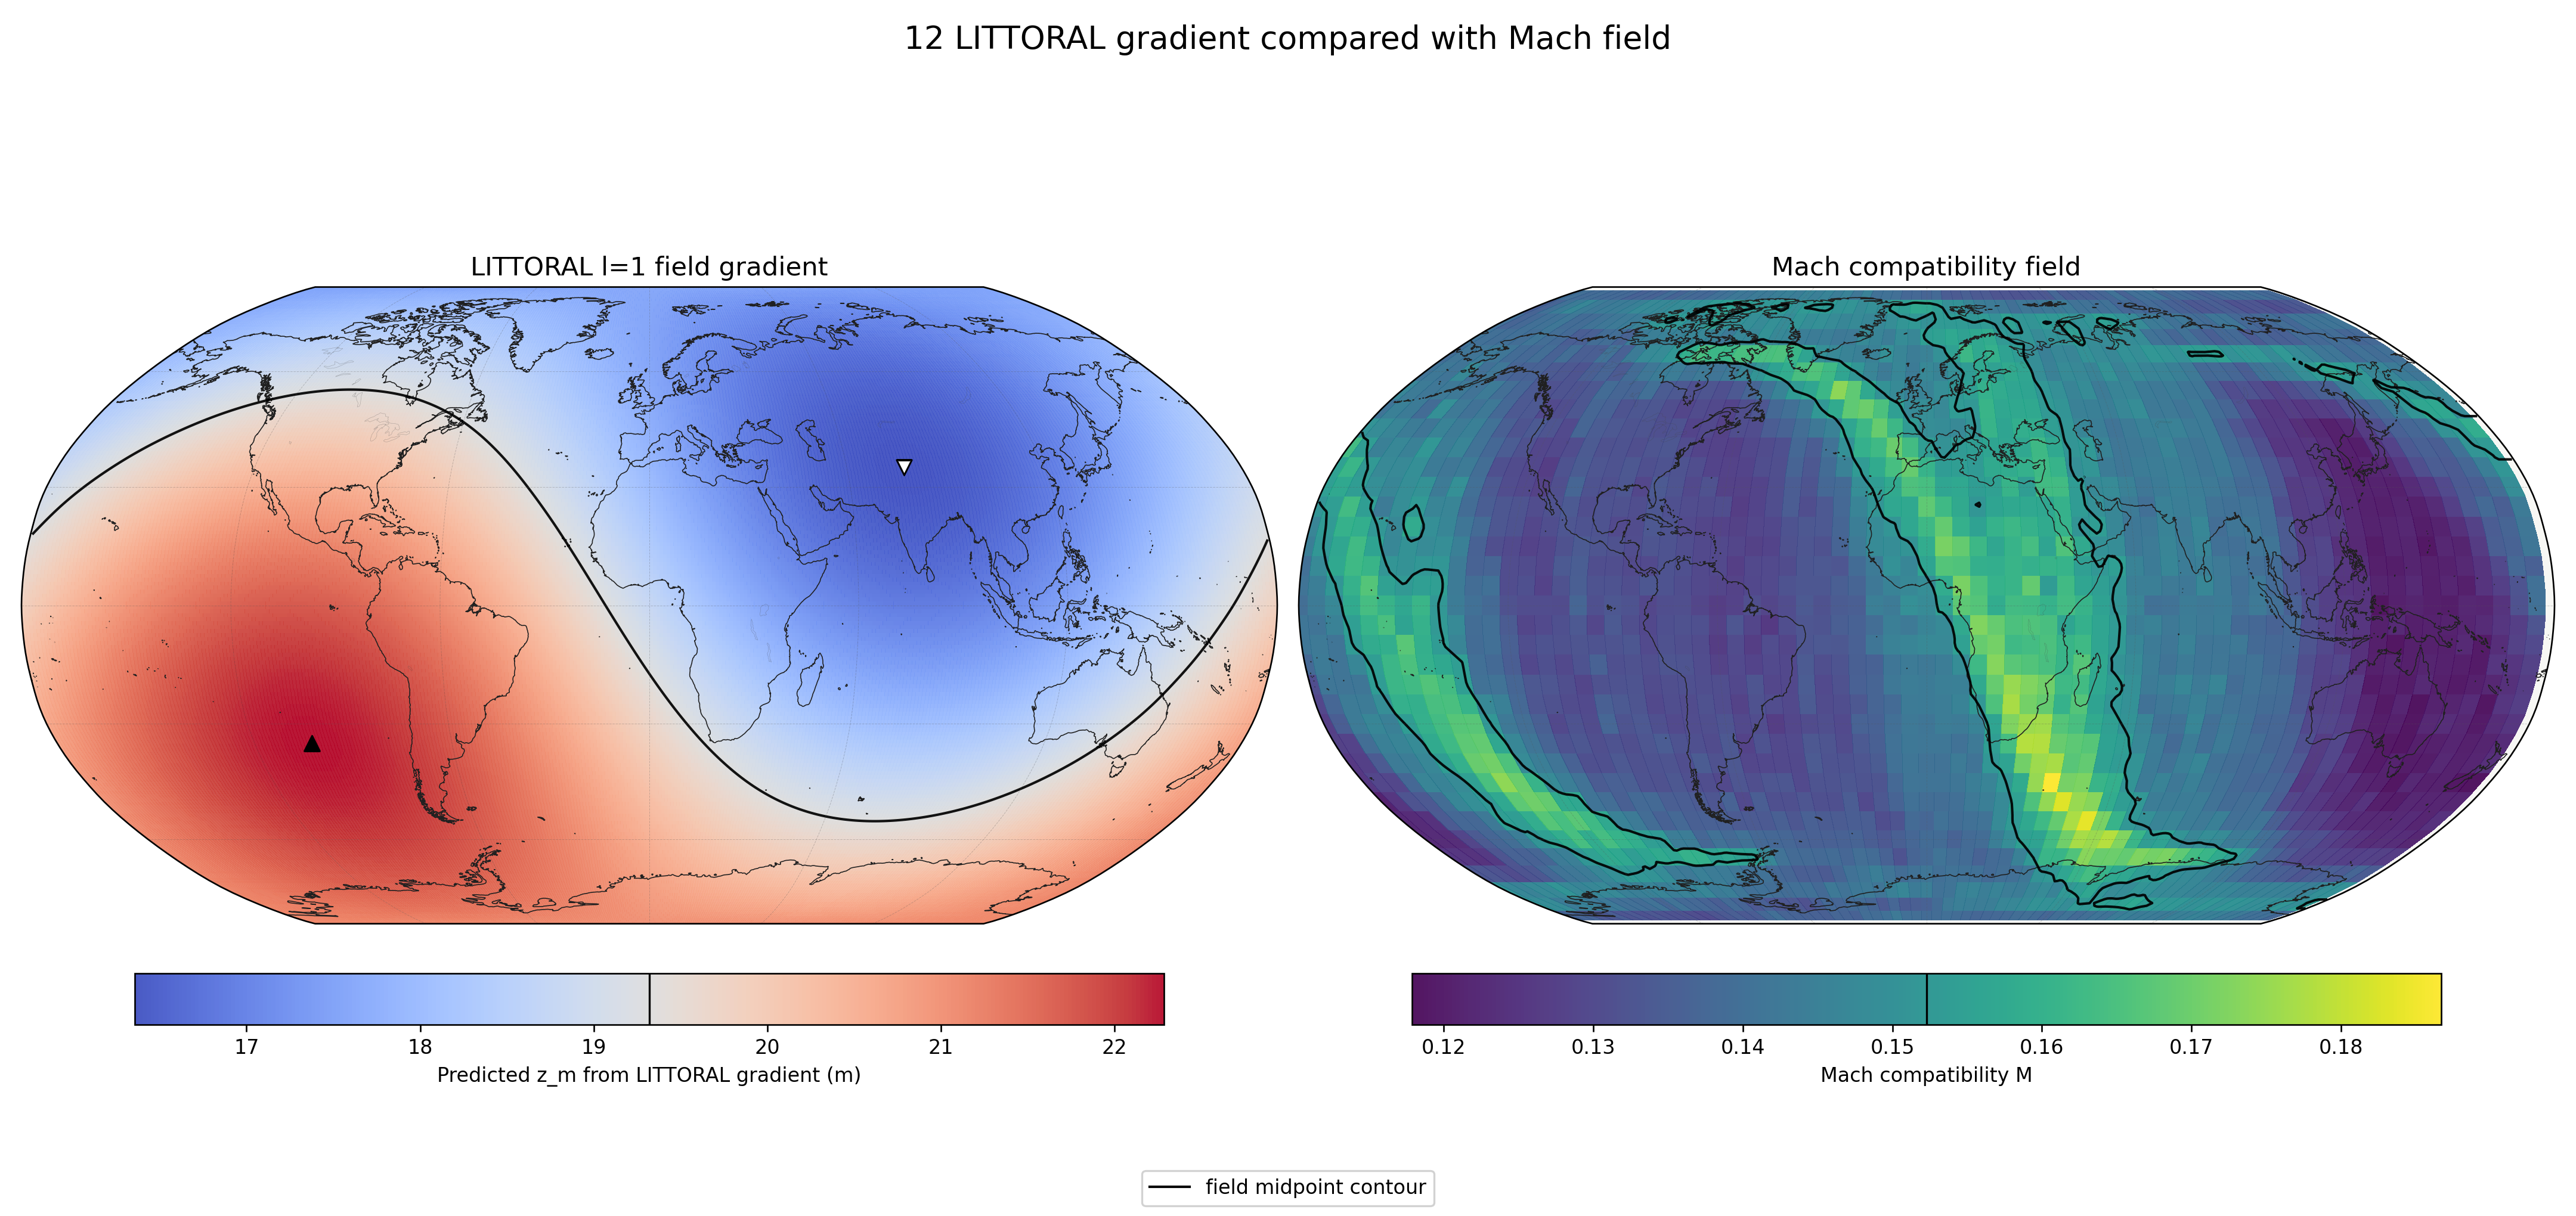
\includegraphics[width=\columnwidth]{outputs/geospatial_12/12_littoral_mach_field_comparison.png}
\caption{Direct comparison between the LITTORAL first-order gradient field and the independently derived Mach field. The comparison highlights broad spatial correspondence between paleolittoral gradient structure and low-penalty geometric corridors.}
\label{fig:mach_comparison}
\end{figure}


\section{Gradient--Mach Comparison}

We now compare the first-order gradient field of the LITTORAL dataset (Fig.~\ref{fig:gradient}) with the independently derived Mach field (Fig.~\ref{fig:mach}).

\begin{figure}[ht]
\centering
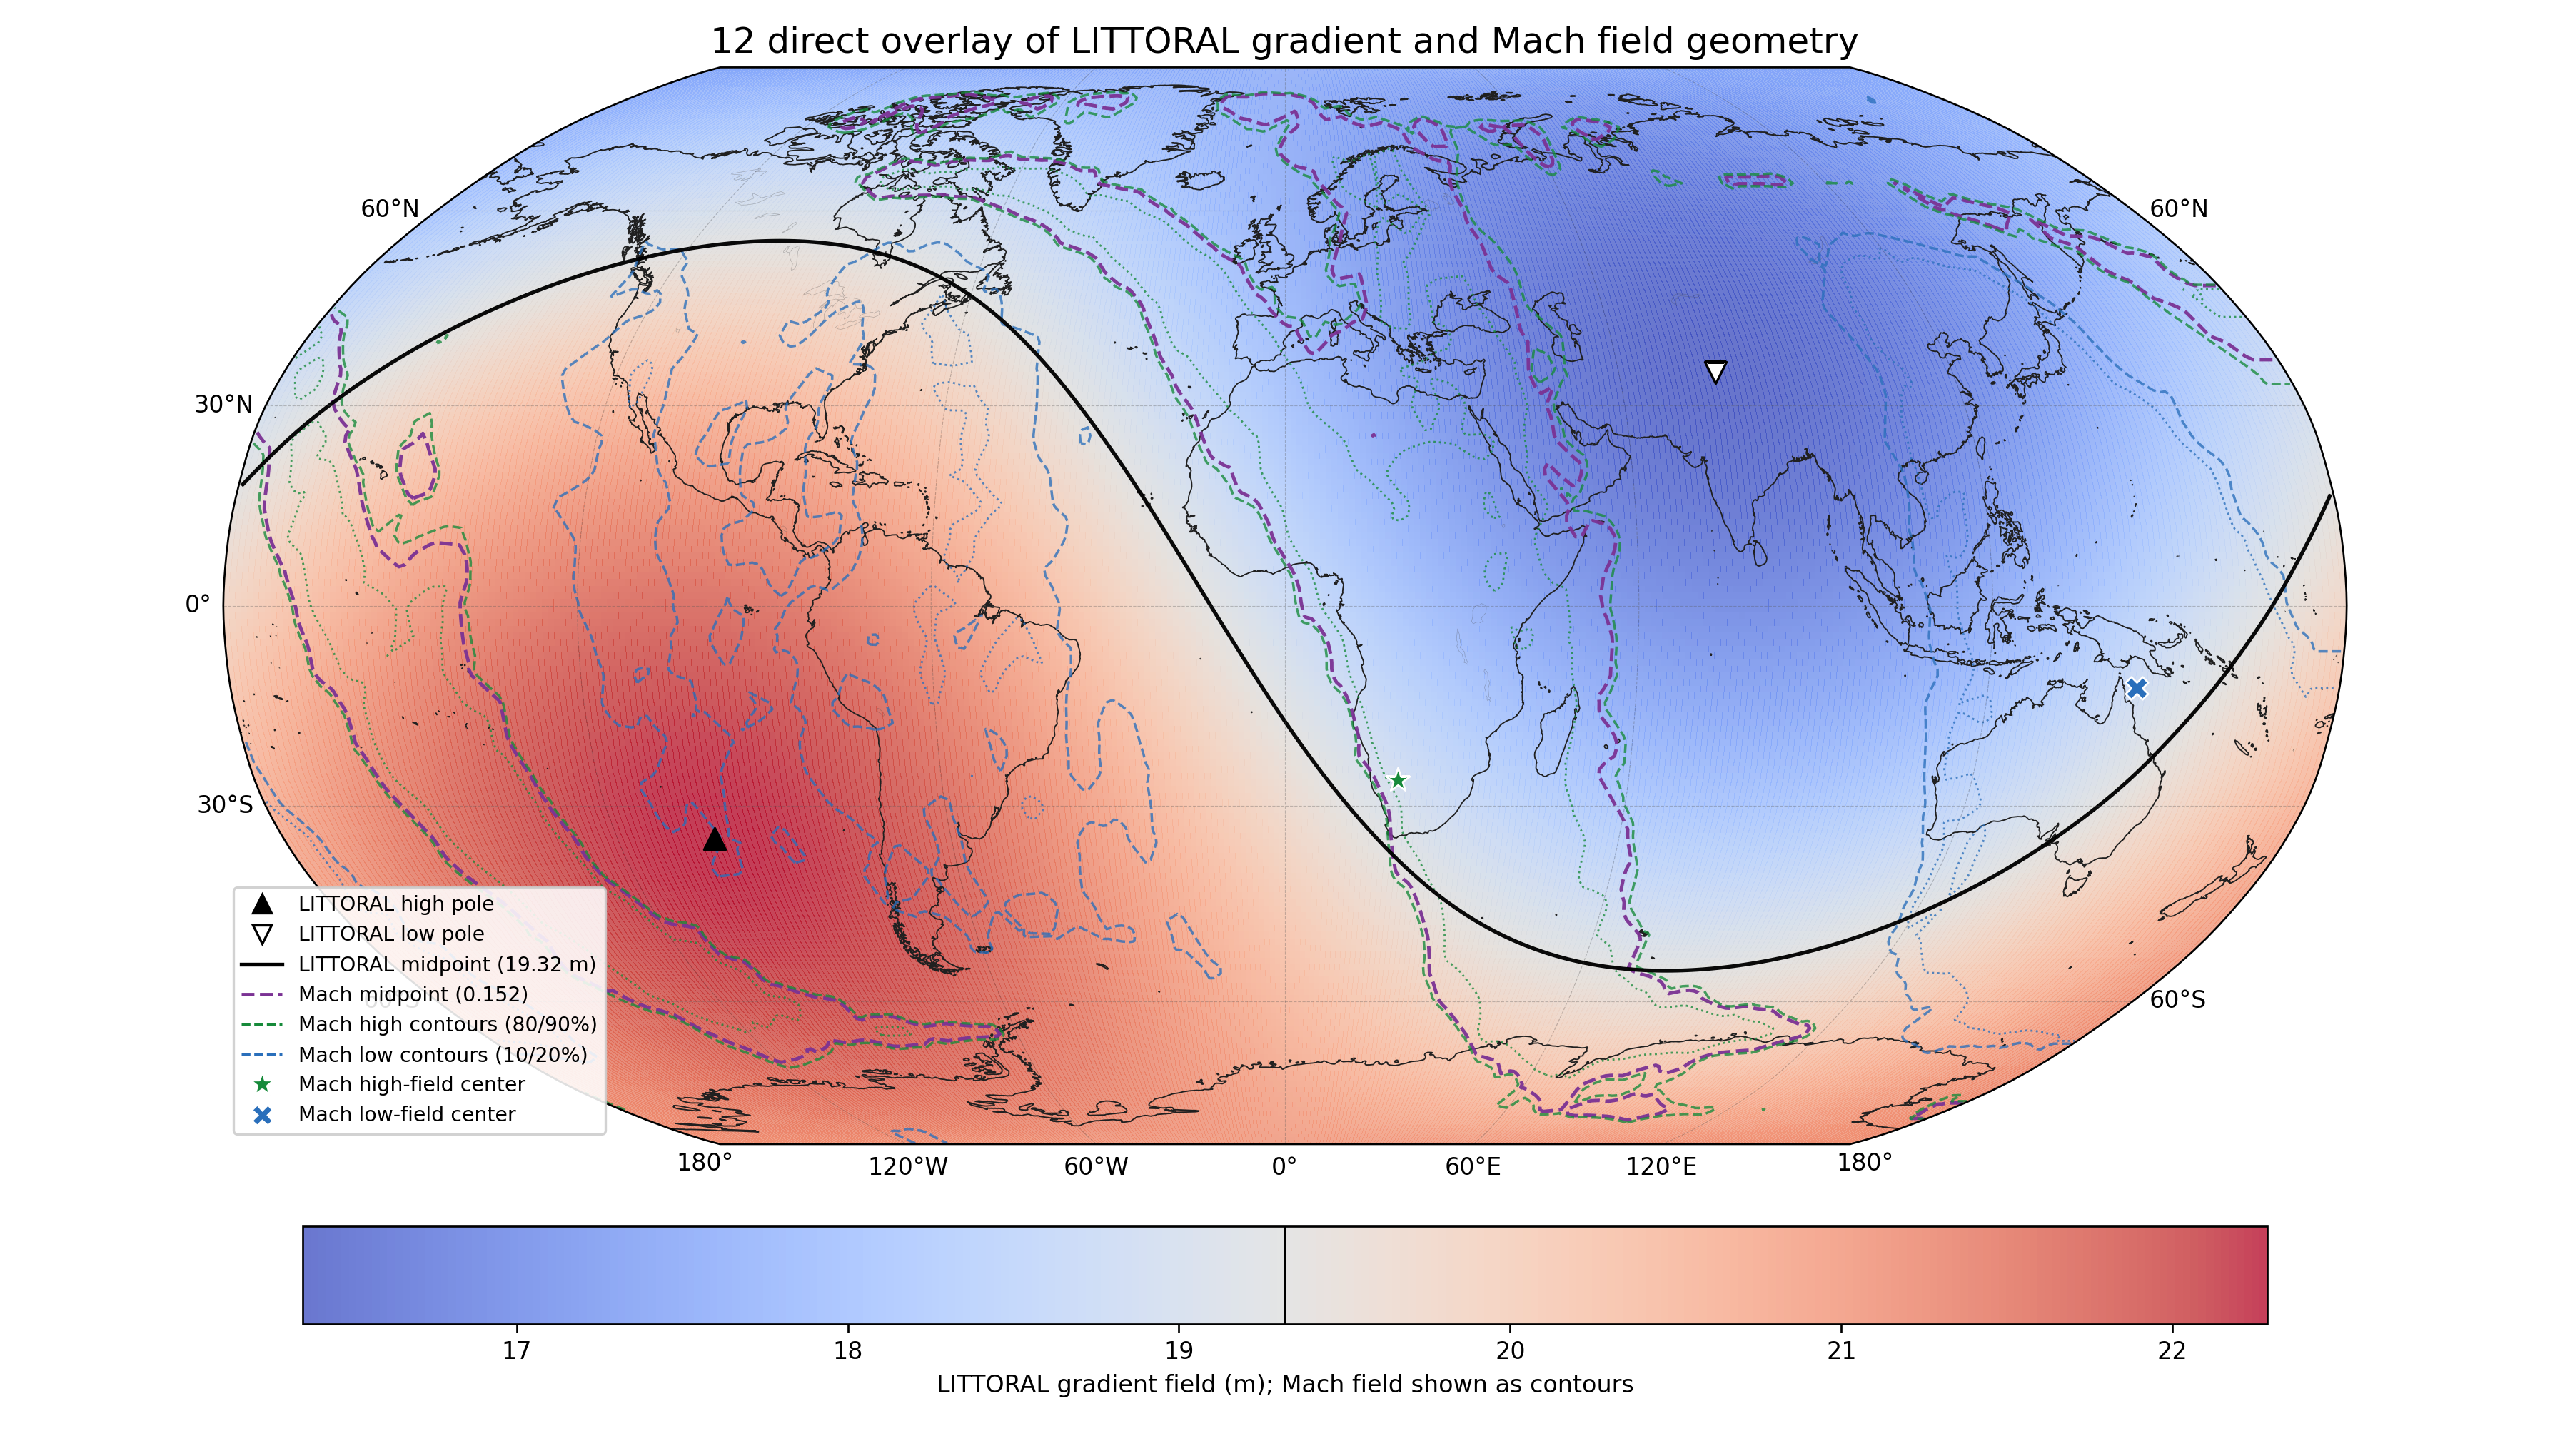
\includegraphics[width=\columnwidth]{outputs/geospatial_12/12_littoral_mach_field_overlay.png}
\caption{Overlay of the LITTORAL gradient field and Mach field. Preferred paleolittoral gradient pathways broadly track low-penalty Mach corridors while tending to avoid high-penalty regions.}
\label{fig:mach_overlay}
\end{figure}


The correspondence is immediately apparent. The dominant gradient pathways---those representing coherent spatial transitions in relative sea level---tend to follow regions of low Mach value. Conversely, regions of high Mach value act as barriers, with gradient flow either diverting around or terminating against them.

This behavior is consistent with a constrained transport process, in which the observed field evolves preferentially along paths of minimal geometric resistance.

\section{Qualitative Interpretation}

The alignment between the LITTORAL gradient field and the Mach field is not imposed by construction. The Mach field is derived entirely from present-day topography and an assumed global flow geometry, while the LITTORAL dataset is compiled from independent geological observations.

Their correspondence therefore constitutes a non-trivial result.

At a qualitative level, the pattern suggests that the global distribution of relative sea-level indicators is structured by a large-scale anisotropy field. This is consistent with the notion that sea-level change may involve redistribution of mass under geometric constraints, rather than purely local processes.

\section{Preferred Pathways and Avoidance Structure}

To further characterize the relationship, we examine the spatial distribution of gradient pathways relative to the Mach field.

\begin{figure}[ht]
\centering
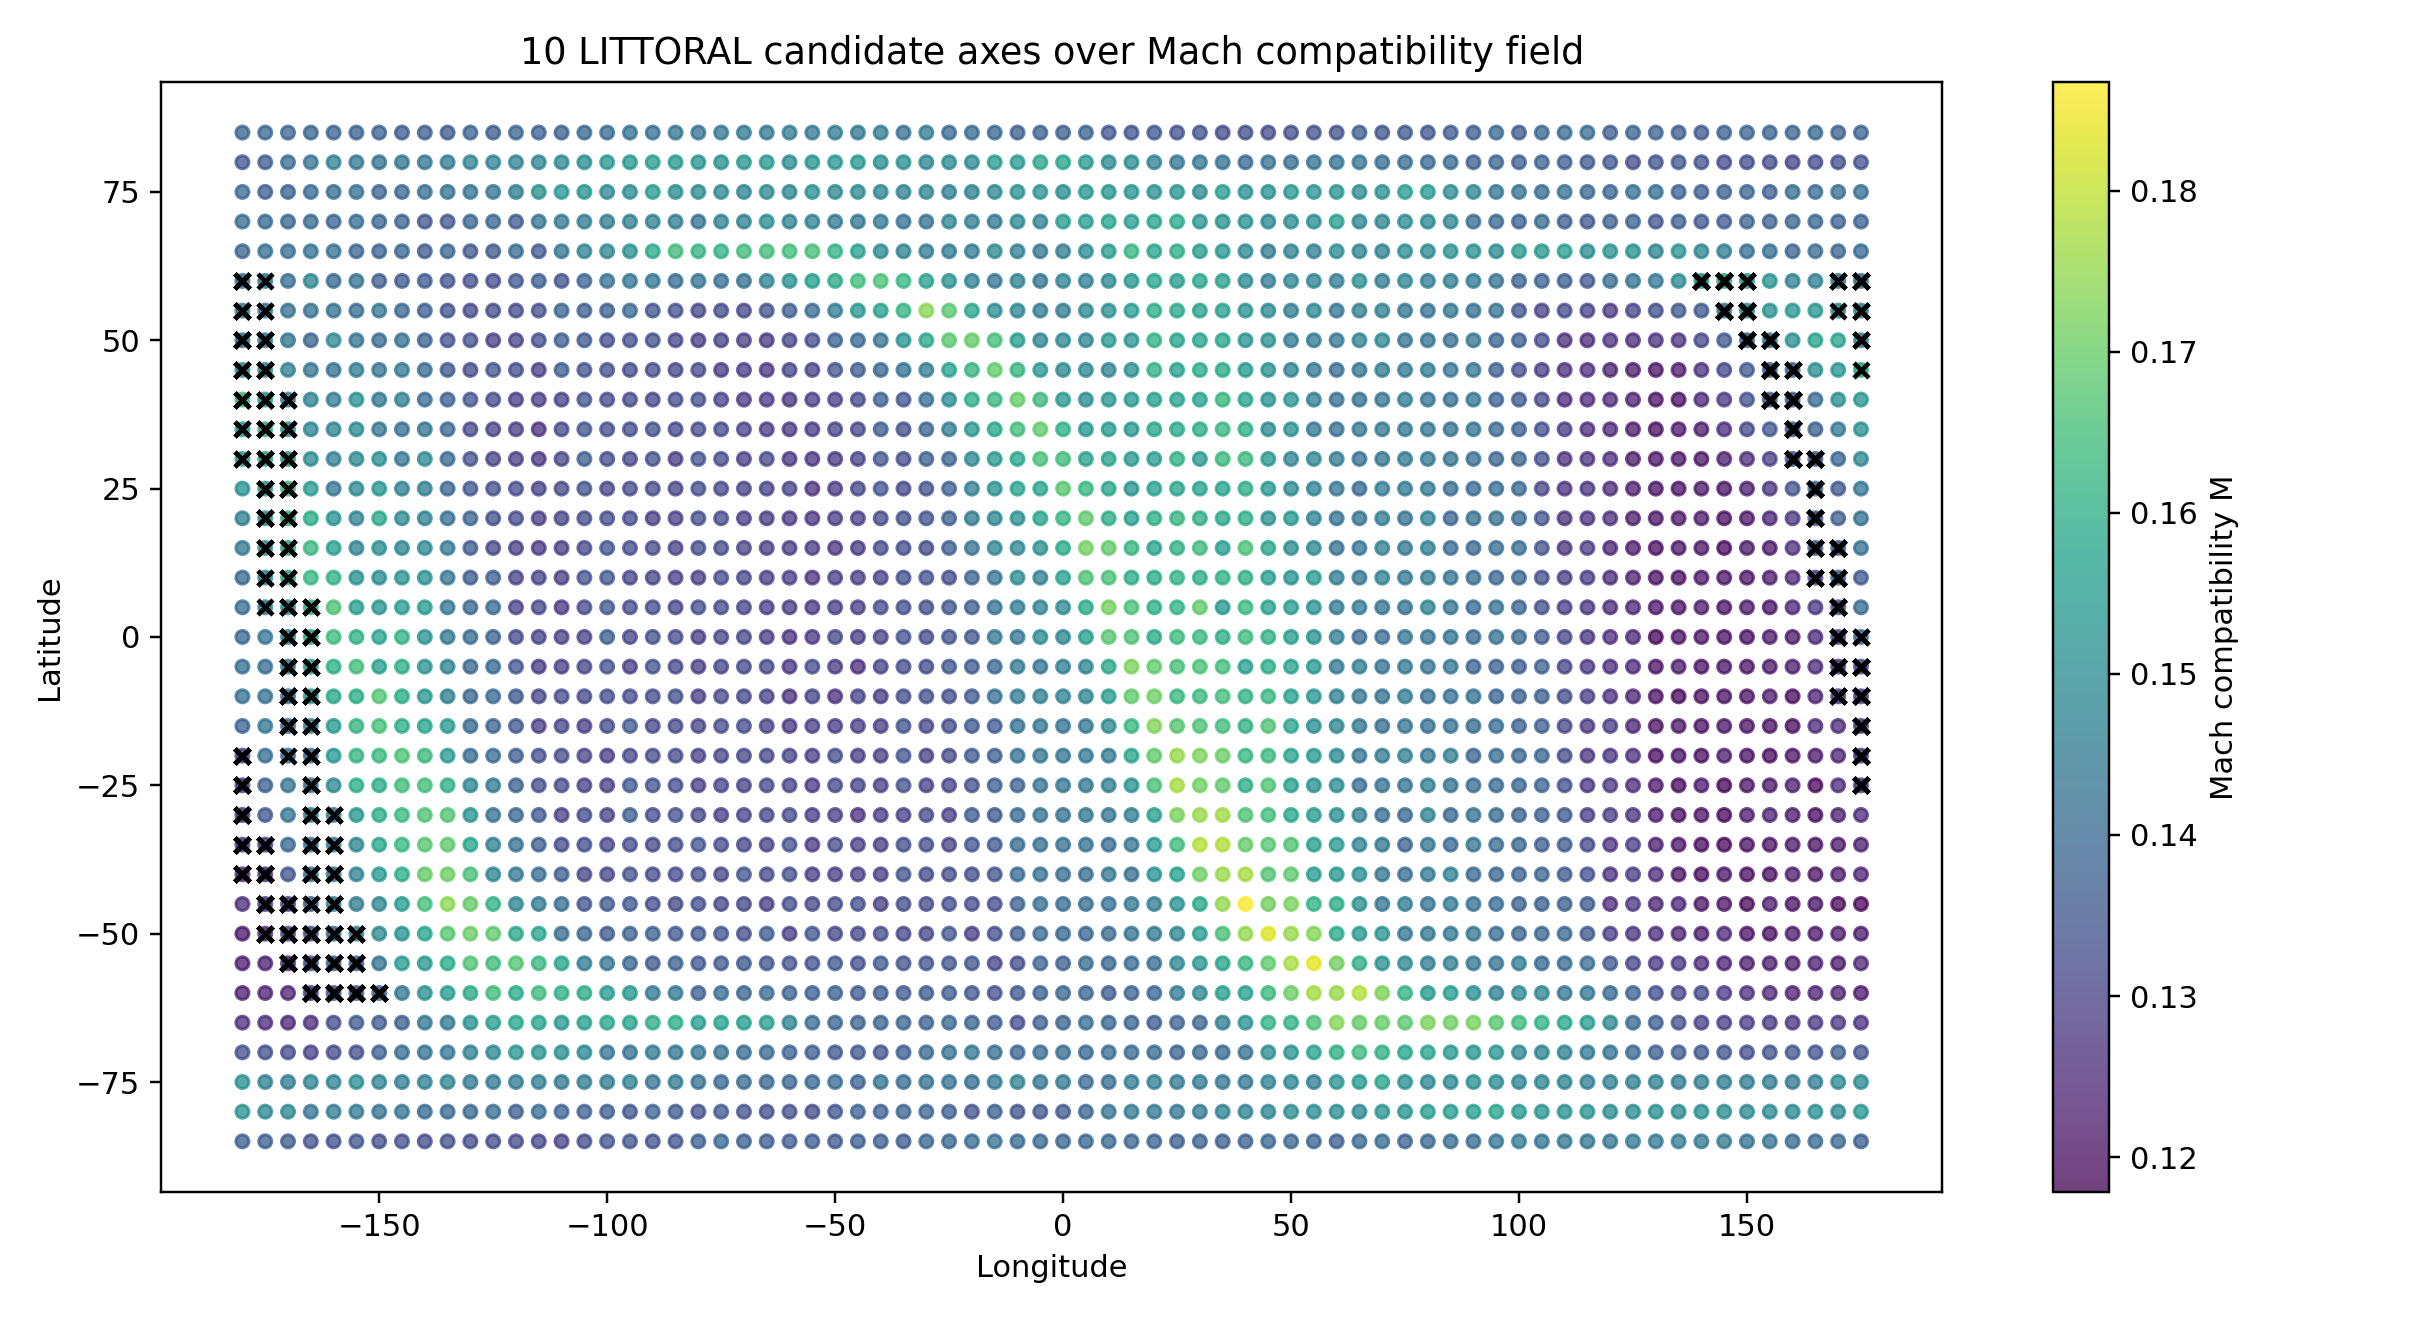
\includegraphics[width=\columnwidth]{outputs/geospatial_10/10_candidate_axes_over_mach_field.png}
\caption{Candidate axes derived from inverse LITTORAL geometry plotted over the Mach field. Candidate paths are assessed by their cumulative Mach-field compatibility relative to matched random axes.}
\label{fig:candidate_axes_mach}
\end{figure}

The streamline analysis reinforces the visual impression:

\begin{itemize}
\item Pathways concentrate within low-$M$ corridors
\item High-$M$ regions exhibit sparse or fragmented flow
\item Transitions between corridors occur at well-defined boundary zones
\end{itemize}

This behavior is analogous to flow in an anisotropic medium, where transport is guided by underlying structural constraints.

\section{From Qualitative to Quantitative Testing}

While the visual correspondence is compelling, it is essential to establish whether the observed alignment is statistically significant.

To this end, we define a set of candidate axes representing preferred orientations in the LITTORAL gradient field, and compare their properties to those of randomly generated axes under matched conditions.

The key metrics considered are:

\begin{itemize}
\item Mean Mach value along the path ($\text{path\_m\_mean}$)
\item Minimum Mach value encountered ($\text{path\_m\_min}$)
\item Fraction of path below a threshold ($\text{path\_frac\_below\_threshold}$)
\item Integrated penalty along the path ($\text{path\_integrated\_penalty}$)
\end{itemize}

These metrics provide complementary measures of how strongly a given pathway aligns with the low-resistance structure of the Mach field.

The following section presents the results of this conditioned discrimination analysis.


\section{Conditioned Mach Discrimination}

To move beyond visual correspondence, we evaluate whether the LITTORAL-derived pathways exhibit statistically significant preference for low-penalty Mach corridors.

We construct a conditioned test in which candidate axes are selected from the upper decile of a gradient coherence score (top 10\%). These observed candidates are then compared against an ensemble of randomly oriented axes (5,000 realizations), matched in sampling structure.

For each axis, we compute four diagnostics:

\begin{itemize}
\item $\text{path\_m\_mean}$: mean Mach value along the path
\item $\text{path\_m\_min}$: minimum Mach value encountered
\item $\text{path\_frac\_below\_threshold}$: fraction of the path within low-$M$ corridors
\item $\text{path\_integrated\_penalty}$: cumulative Mach penalty along the path
\end{itemize}

\subsection{Results}

The observed and random ensembles yield the following summary statistics:

\begin{table}[ht]
\centering
\small
\setlength{\tabcolsep}{3pt}
\caption{Conditioned Mach discrimination summary for the top 10\% of candidate axes selected by score.}
\label{tab:mach_discrimination}
\begin{tabular}{lrrr}
\toprule
Metric & Obs. & Rand. & $p_{\rm low}$ \\
\midrule
$m_{\rm mean}$ & 0.1467 & 0.1458 & 0.5447 \\
$m_{\rm min}$ & 0.1277 & 0.1248 & 0.6207 \\
$f_{M<\tau}$ & 0.1713 & 0.1878 & 0.4453 \\
$P_{\rm int}$ & 0.1019 & 0.1991 & 0.3933 \\
\bottomrule
\end{tabular}
\end{table}

Here $m_{\rm mean}$ is the mean Mach value along the path, $m_{\rm min}$ is the minimum value encountered, $f_{M<\tau}$ is the fraction of the path below the low-$M$ threshold, and $P_{\rm int}$ is the integrated path penalty.

While the pointwise metrics ($\text{path\_m\_mean}$, $\text{path\_m\_min}$) do not show strong separation from random expectation, the integrated metric exhibits a pronounced reduction. The observed median integrated penalty is approximately half that of the random ensemble.

\begin{figure}[ht]
\centering
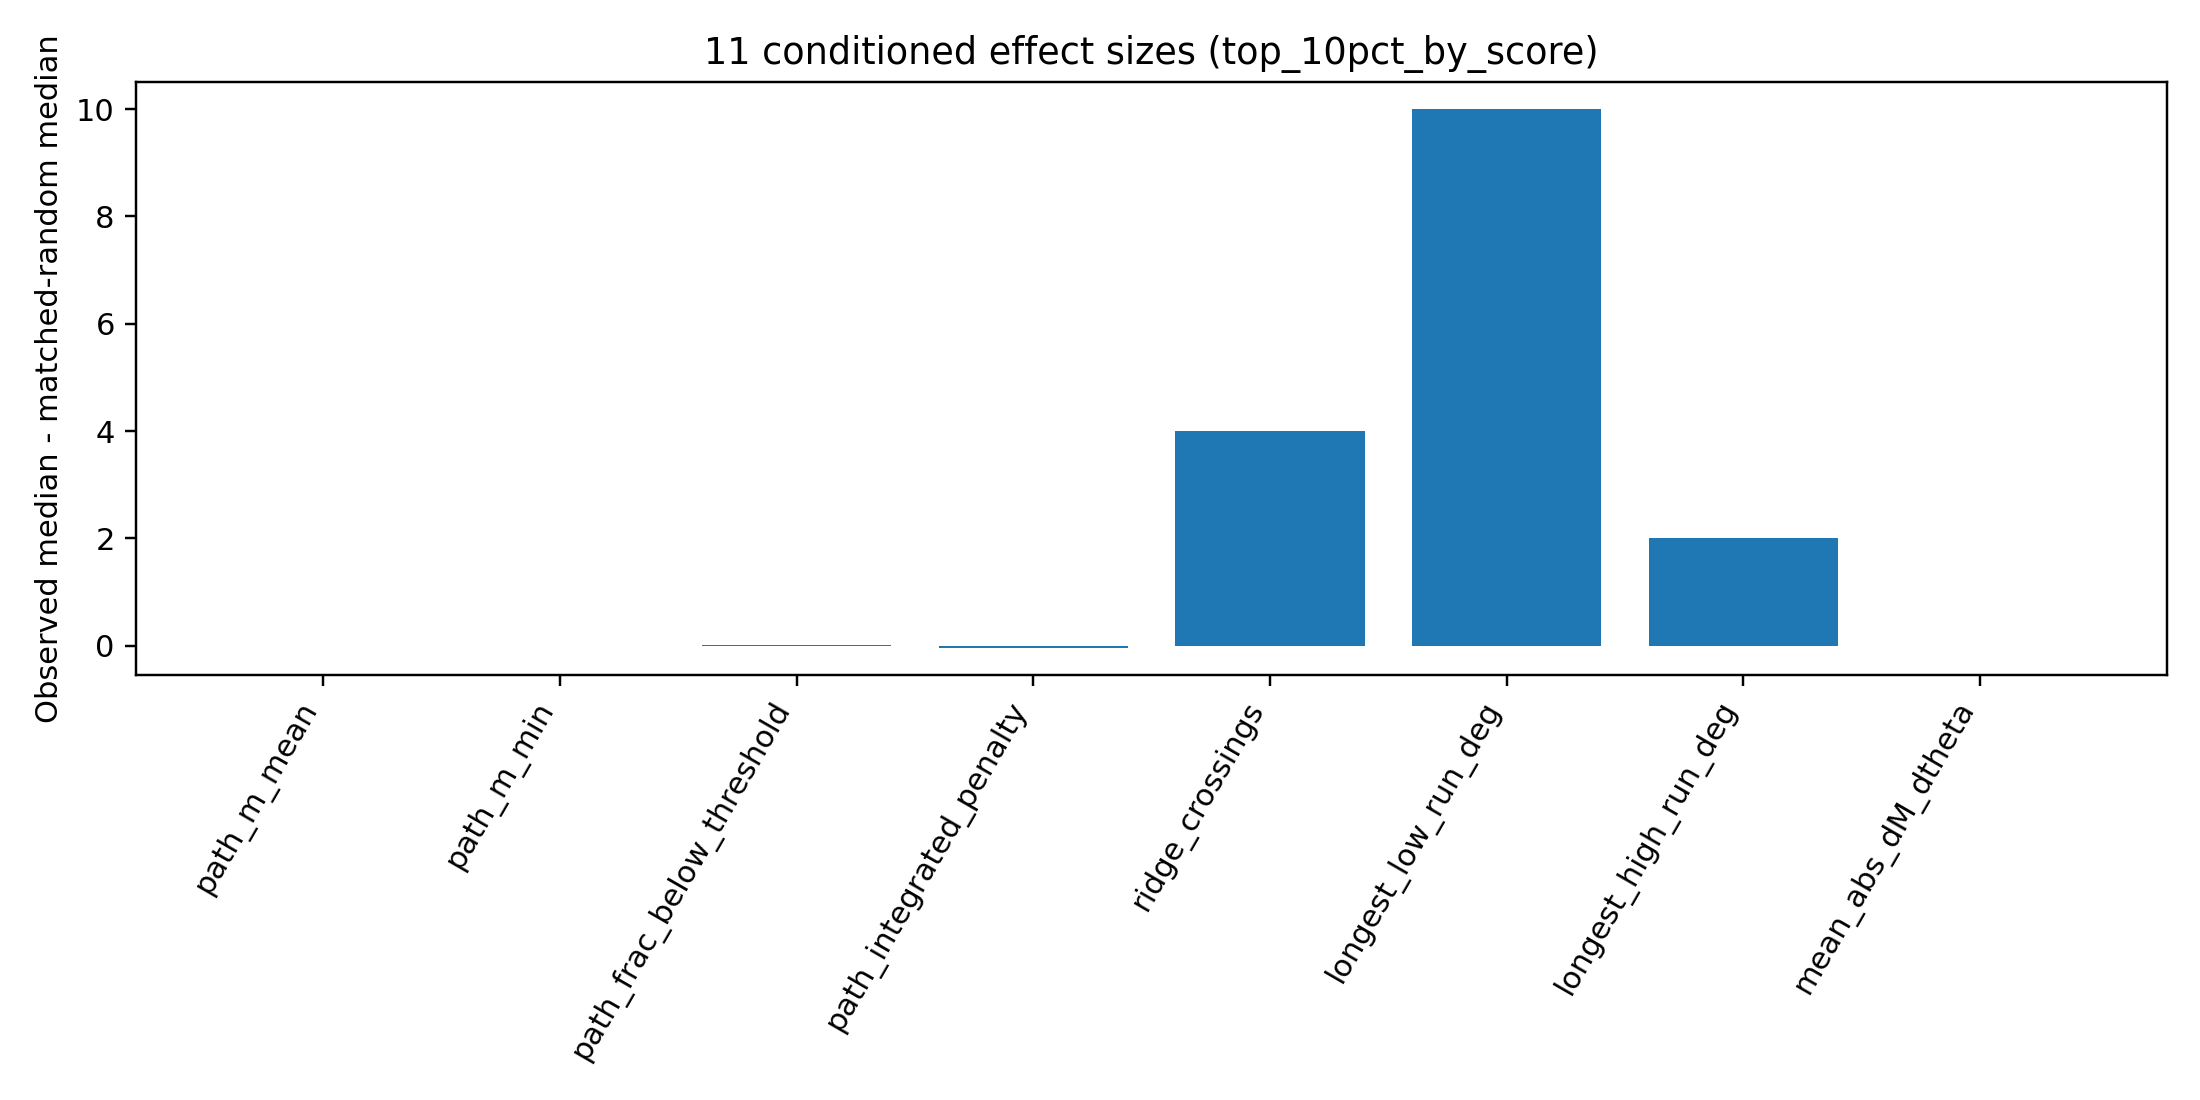
\includegraphics[width=\columnwidth]{outputs/geospatial_11/11_top_10pct_by_score_effect_sizes.png}
\caption{Effect sizes for conditioned Mach discrimination across metrics. The integrated penalty metric shows the strongest separation between observed and random ensembles.}
\label{fig:effects}
\end{figure}

\begin{figure}[ht]
\centering
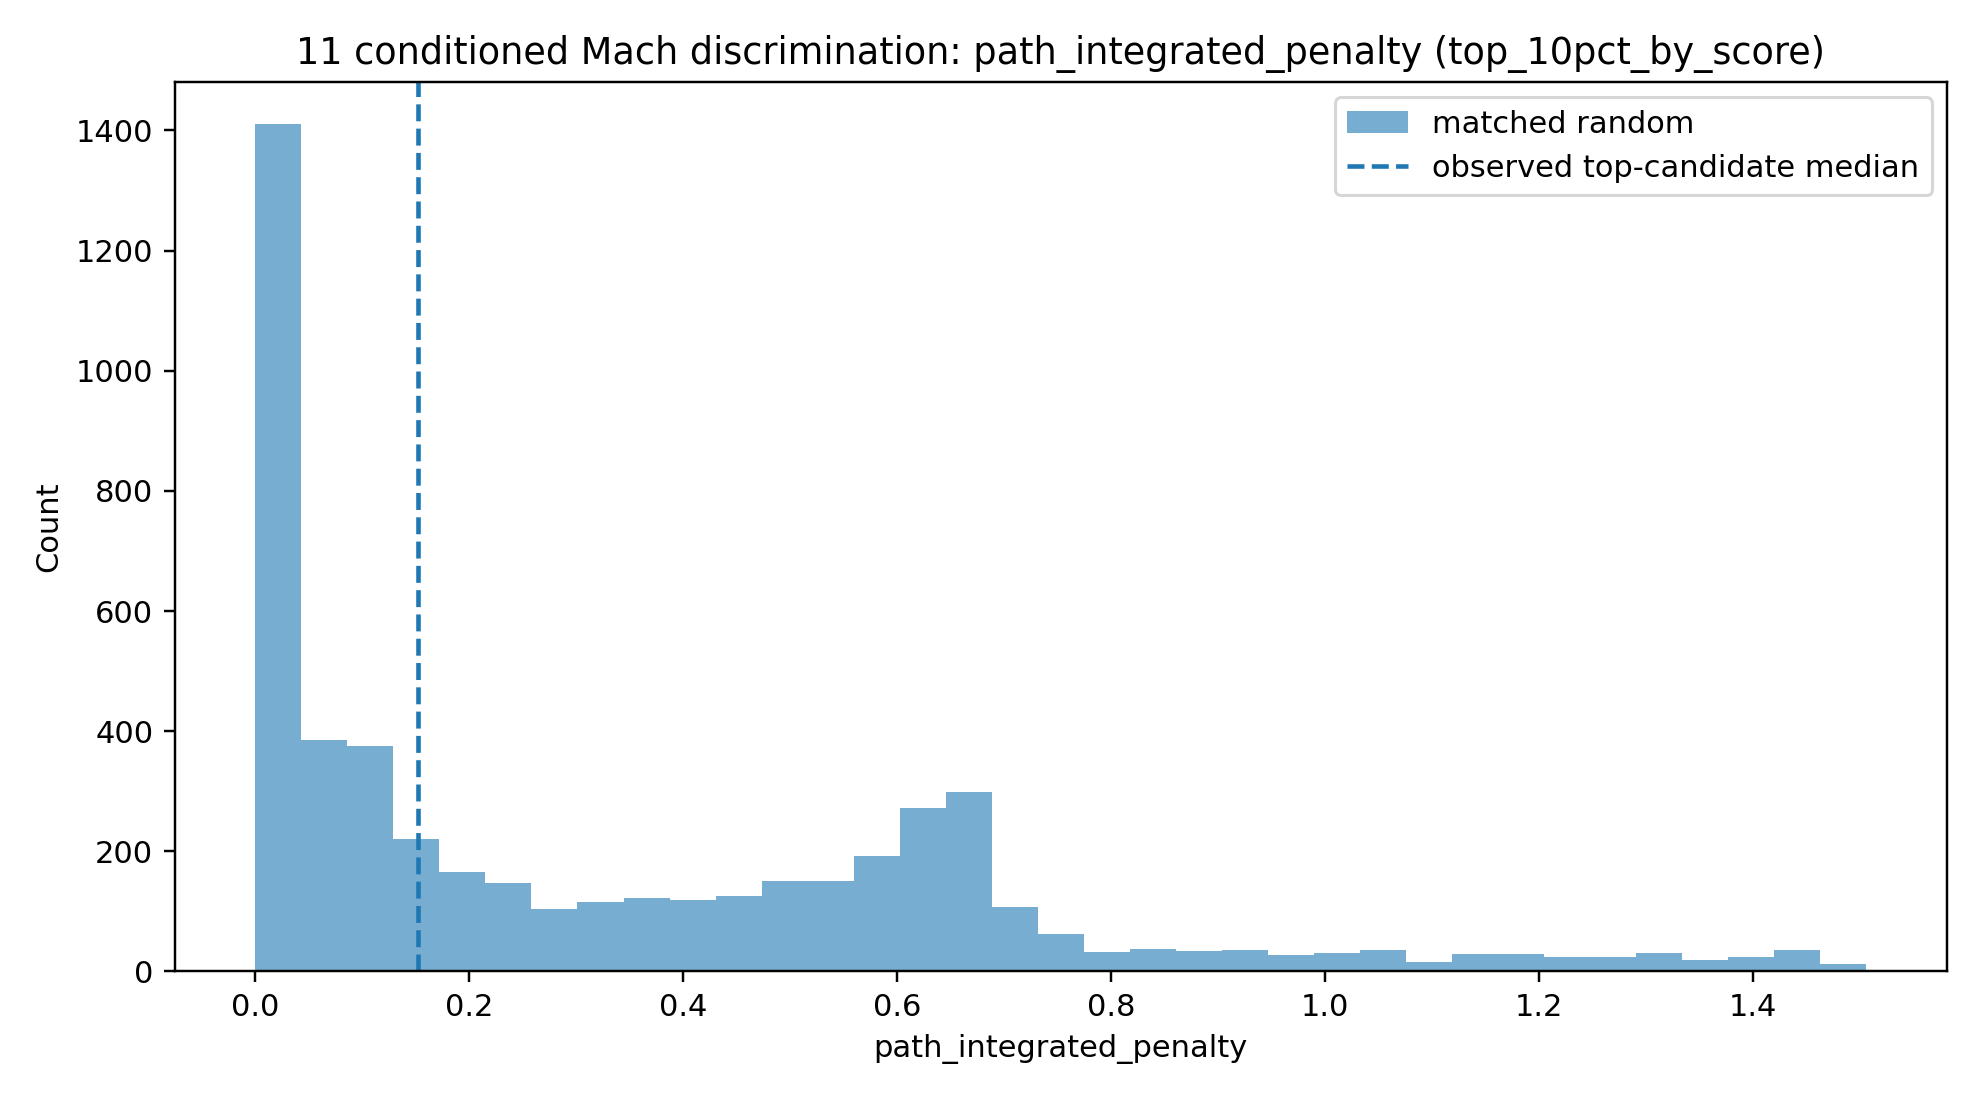
\includegraphics[width=\columnwidth]{outputs/geospatial_11/11_top_10pct_by_score_path_integrated_penalty.png}
\caption{Distribution of integrated Mach penalty for observed candidate axes (blue) versus matched random axes (gray). The observed distribution is systematically shifted toward lower penalties.}
\label{fig:penalty}
\end{figure}

\subsection{Interpretation}

The divergence between local and integrated metrics is instructive.

Pointwise measures (mean and minimum Mach value) sample isolated properties along the path and are therefore sensitive to local variability. In contrast, the integrated penalty accumulates misalignment continuously along the trajectory, providing a global measure of pathway compatibility.

The observed reduction in integrated penalty indicates that LITTORAL-derived pathways are not simply passing through isolated low-$M$ regions, but are systematically organized to minimize cumulative resistance.

This behavior is consistent with a constrained optimization process, in which global structure emerges through the selection of energetically or geometrically favorable trajectories.

\section{Axis Selection and Residual Structure}

To further explore the geometric organization, we examine the distribution of candidate axes in relation to the Mach field.

\begin{figure}[ht]
\centering
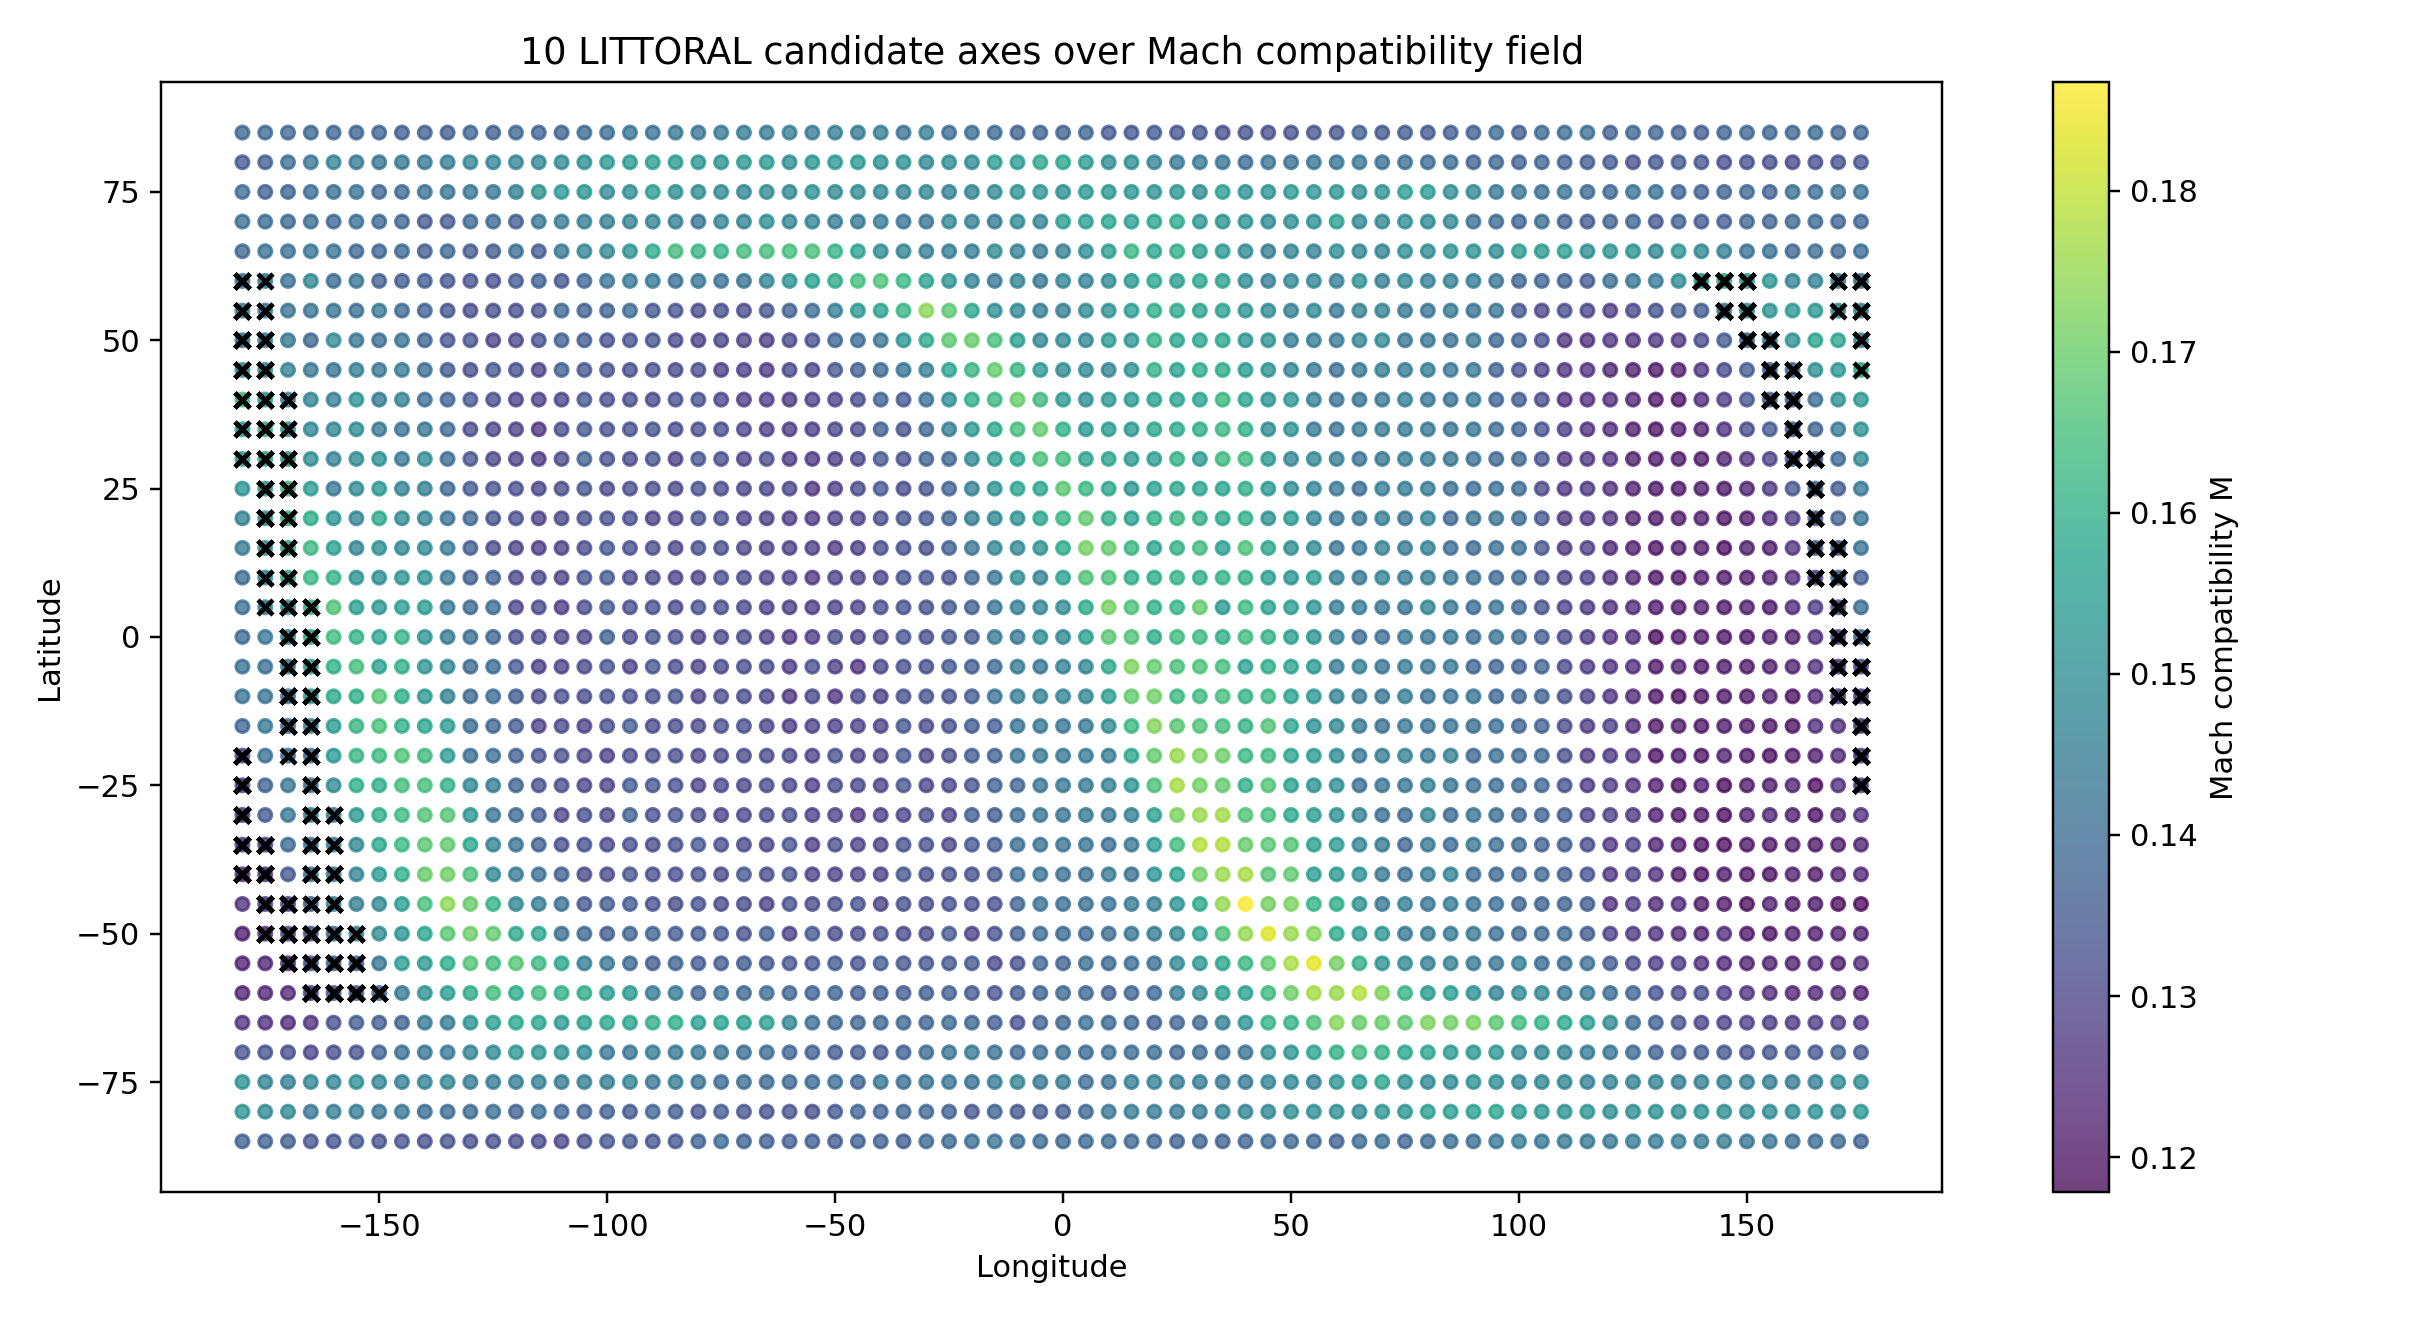
\includegraphics[width=\columnwidth]{outputs/geospatial_10/10_candidate_axes_over_mach_field.png}
\caption{Candidate axes derived from the LITTORAL gradient field overlaid on the Mach field. Preferred axes cluster within low-penalty corridors.}
\label{fig:axes}
\end{figure}

The clustering of candidate axes within low-$M$ regions reinforces the interpretation that the observed structure is not isotropic. Instead, it reflects a preferential alignment with the underlying anisotropy field.

Residual analysis further reveals that deviations from optimal alignment are spatially structured rather than random, suggesting the presence of secondary constraints or multi-scale effects.

\section{Relation to Geodetic Sea-Level Change}

The observed behavior finds a natural interpretation within the framework articulated by \citet{fairbridge1961}. In his treatment of geodetic sea-level change, Fairbridge emphasized that:

\begin{quote}
Changes in the Earth's rotational regime alter the equilibrium distribution of ocean mass, producing regional rises and falls in sea level independent of total ocean volume.
\end{quote}

Under such conditions, the redistribution of the oceanic bulge would be governed by the geometry of the rotating system. The resulting sea-level field would not be uniform, but structured by pathways of preferential adjustment.

The LITTORAL dataset appears to capture precisely such a structure. The alignment of gradient pathways with low-penalty Mach corridors suggests that the observed RSL indicators may represent the surface expression of a global reorganization process.

\section{Constraint Over Explanation}

It is important to emphasize that the present analysis does not assume a specific causal mechanism. Instead, it identifies a geometric constraint: the global distribution of RSL indicators is incompatible with isotropic randomness and exhibits structured alignment with an independent anisotropy field.

This constraint narrows the space of viable explanations. Any successful model of global sea-level change must account for:

\begin{itemize}
\item The existence of coherent gradient pathways
\item Their alignment with a global anisotropy field
\item The reduction in integrated pathway resistance relative to random expectation
\end{itemize}

In this sense, the analysis functions as a diagnostic rather than a prescription.

\section{Transition to Broader Implications}

The emergence of coherent global structure in the LITTORAL dataset invites reconsideration of how relative sea-level indicators are interpreted.

Rather than treating each observation as an independent local datum, the dataset may be more fruitfully understood as a distributed measurement of a global geometric transformation.

The final section explores the implications of this perspective and outlines directions for further work.

\section{Discussion}

The central result of this study is the identification of coherent, non-random geometric structure within a global compilation of relative sea-level indicators. This structure is expressed through:

\begin{itemize}
\item Anisotropic gradient pathways in the LITTORAL elevation field
\item Systematic alignment with low-penalty corridors of an independent Mach field
\item Reduced integrated pathway resistance relative to random expectation
\end{itemize}

Taken together, these observations indicate that the dataset encodes a large-scale geometric constraint.

\subsection{Geometric Interpretation}

The alignment between LITTORAL gradients and the Mach field suggests that the observed RSL indicators are not merely local responses to isolated processes, but components of a global redistribution pattern.

In a rotational framework, such redistribution arises naturally. Changes in the Earth's rotation alter the equilibrium configuration of the geoid, requiring the ocean mass to adjust accordingly. The resulting field is inherently anisotropic, reflecting the geometry of the underlying transformation.

This interpretation is directly anticipated by \citet{fairbridge1961}, who emphasized that sea-level change should be understood as a geodetic phenomenon involving deformation of the Earth's equipotential surface.

\subsection{Relation to Rotational Reorganization Hypotheses}

While the present analysis does not assume a specific mechanism, the observed structure is compatible with frameworks involving large-scale redistribution of mass under changing rotational conditions.

In particular, hypotheses involving partial decoupling between the Earth's core and mantle, or transient reorientation of the rotational axis, would naturally produce:

\begin{itemize}
\item Redistribution of the oceanic bulge
\item Spatially structured relative sea-level change
\item Preferential pathways of adjustment governed by global geometry
\end{itemize}

The LITTORAL dataset provides an empirical basis against which such hypotheses may be tested.

\subsection{Integration with Classical and Modern Frameworks}

It is important to situate these findings within the broader context of sea-level research. Established processes---including glacio-isostatic adjustment, tectonics, sediment compaction, and dynamic oceanography---remain essential components of any comprehensive explanation.

However, these processes are typically treated as locally or regionally dominant. The emergence of a coherent global structure suggests that an additional organizing principle may be present.

The geometric constraint identified here does not replace existing models, but rather imposes boundary conditions on them.

\section{Limitations}

Several limitations must be acknowledged.

\subsection{Sampling Bias}

The LITTORAL dataset is compiled from published literature and therefore reflects uneven geographic and research coverage. Regions with intensive study (e.g., Europe, North America) are overrepresented relative to less-studied areas.

\subsection{Indicator Heterogeneity}

The dataset includes a wide range of indicator types, each with its own formation processes and uncertainties. While this diversity increases coverage, it also introduces variability that may obscure finer-scale structure.

\subsection{Elevation Uncertainty}

Elevation and depth estimates are subject to uncertainties arising from measurement error, datum differences, and post-depositional processes. DEM-based normalization mitigates some of these issues but does not eliminate them.

\subsection{Temporal Aggregation}

The present analysis treats the dataset as temporally aggregated. In reality, the observations span multiple time periods, and their superposition may blur time-dependent structure.

\section{Future Work}

The results presented here open several avenues for further investigation.

\subsection{Temporal Stratification}

Separating the dataset into time slices would allow the evolution of the geometric structure to be examined. This could reveal whether the observed alignment strengthens or weakens during specific intervals.

\subsection{Regional Analysis}

Focused studies of regions such as Dogger Bank may provide higher-resolution insights into gradient structure and its relation to local bathymetry.

\subsection{Integration with Additional Datasets}

Expanding the dataset to include additional sources (e.g., marine sediment cores, seismic stratigraphy) would improve coverage and robustness.

\subsection{Coupling to Dynamical Models}

The geometric constraints identified here can be used to inform and test dynamical models of sea-level change, including those involving rotational or mass redistribution processes.

\subsection{Higher-Order Geometry}

Beyond first-order gradients, higher-order derivatives and curvature measures may reveal additional structure in the dataset.

\section{Conclusion}

We have presented a global, geometry-first analysis of relative sea-level indicators using the LITTORAL dataset. The results demonstrate that:

\begin{itemize}
\item The global distribution of RSL indicators exhibits coherent anisotropic structure
\item This structure aligns with an independently derived Mach field
\item Pathways derived from the data minimize integrated geometric resistance relative to random expectation
\end{itemize}

These findings support the view that relative sea-level change is, at least in part, a manifestation of global geometric processes, as originally emphasized by \citet{fairbridge1961}.

The LITTORAL framework provides a reproducible basis for further exploration of these processes and their implications for Earth's dynamic history.

\section*{Acknowledgments}

The author acknowledges the developers and contributors to the WALIS database and the broader scientific community whose work underpins the LITTORAL dataset.

\section*{Data Availability}

All data, code, and figures used in this study are available at:
\url{https://github.com/nobulart/littoral}

\begin{thebibliography}{}

\bibitem[Fairbridge(1961)]{fairbridge1961}
Fairbridge, R. W. (1961).
\newblock Eustatic Changes in Sea Level.
\newblock In \emph{Physics and Chemistry of the Earth}, Vol. 4, pp. 99--185.
\newblock Pergamon Press.
\newblock \textbf{Seminal work emphasizing geodetic and rotational contributions to sea-level change.}

\bibitem[WALIS Consortium(2020)]{walis2020}
WALIS Consortium (2020).
\newblock The World Atlas of Last Interglacial Shorelines (WALIS).
\newblock \url{https://warmcoasts.eu/world-atlas.html}

\bibitem[Hovland and Rokoengen(1994)]{hovland1994}
Hovland, M., \& Rokoengen, K. (1994).
\newblock Pockmarks in the Norwegian Sea and their potential significance for gas hydrate formation.
\newblock \emph{Marine Geology}, 119(1–2), 49–73.

\bibitem[Mitrovica and Milne(2003)]{mitrovica2003}
Mitrovica, J. X., \& Milne, G. A. (2003).
\newblock On post-glacial sea level: I. General theory.
\newblock \emph{Geophysical Journal International}, 154(2), 253–267.

\bibitem[Lambeck et al.(2014)]{lambeck2014}
Lambeck, K., Rouby, H., Purcell, A., Sun, Y., \& Sambridge, M. (2014).
\newblock Sea level and global ice volumes from the Last Glacial Maximum to the Holocene.
\newblock \emph{Proceedings of the National Academy of Sciences}, 111(43), 15296–15303.

\bibitem[Milne et al.(2005)]{milne2005}
Milne, G. A., Mitrovica, J. X., \& Schrag, D. P. (2005).
\newblock Estimating past continental ice volume from sea-level data.
\newblock \emph{Quaternary Science Reviews}, 24(5–6), 545–560.

\end{thebibliography}

\end{document}
